\subsection{Klassifizierung von Signalen S.7}
\begin{table}[H]
\centering
\renewcommand{\arraystretch}{1.1}
\begin{tabularx}{\textwidth}{|>{\centering\arraybackslash}X|>{\centering\arraybackslash}X|}
\hline

\begin{minipage}[t]{\linewidth}\centering
\textbf{Energiesignal}\\[2pt]
$\displaystyle E=\int_{-\infty}^{\infty}|x(t)|^2\,dt < \infty$\\[2pt]
Endliche Energie\\[4pt]
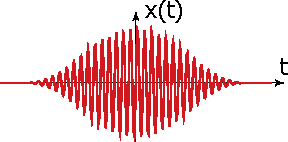
\includegraphics[width=0.65\linewidth]{chapters/03_Signale/figures/energiesignal.pdf}
\end{minipage}
&
\begin{minipage}[t]{\linewidth}\centering
\textbf{Leistungssignal}\\[2pt]
$\displaystyle P=\lim_{T\to\infty}\frac{1}{T}\int_{-T/2}^{T/2}|x(t)|^2\,dt < \infty$\\[2pt]
Unendliche Energie\\[4pt]
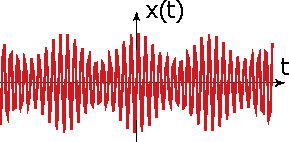
\includegraphics[width=0.65\linewidth]{chapters/03_Signale/figures/leistungssignal.pdf}
\end{minipage}
\\ \hline

\begin{minipage}[t]{\linewidth}\centering
\textbf{aperiodisches Signal}\\[2pt]
$x(t) \neq x(t+n\cdot T)$\\[4pt]
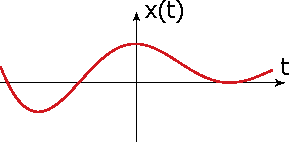
\includegraphics[width=0.65\linewidth]{chapters/03_Signale/figures/aperiodischessignal.pdf}
\end{minipage}
&
\begin{minipage}[t]{\linewidth}\centering
\textbf{periodisches Signal}\\[2pt]
$x(t) = x(t+n\cdot T)$\\[4pt]
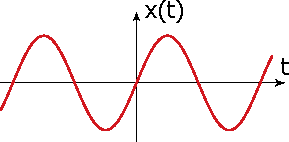
\includegraphics[width=0.65\linewidth]{chapters/03_Signale/figures/periodischessignal.pdf}
\end{minipage}
\\ \hline

\begin{minipage}[t]{\linewidth}\centering
\textbf{deterministisches Signal}\\[2pt]
$x(t)=f(t)$, Verlauf ist bekannt\\[4pt]
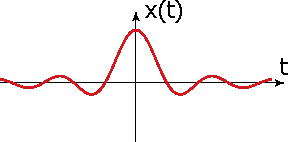
\includegraphics[width=0.65\linewidth]{chapters/03_Signale/figures/deterministischessignal.pdf}
\end{minipage}
&
\begin{minipage}[t]{\linewidth}\centering
\textbf{stochastisches Signal}\\[2pt]
Signalverlauf ist unbekannt bzw. zufällig\\[4pt]
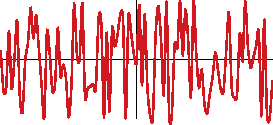
\includegraphics[width=0.65\linewidth]{chapters/03_Signale/figures/stochastischessignal.pdf}
\end{minipage}
\\ \hline

\begin{minipage}[t]{\linewidth}\centering
\textbf{zeitkontinuierliches Signal}\\[2pt]
$x(t)$ ist immer definiert\\[4pt]
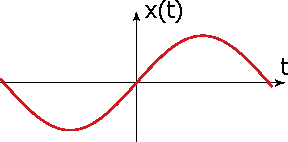
\includegraphics[width=0.65\linewidth]{chapters/03_Signale/figures/zeitkontinuierlichessignal.pdf}
\end{minipage}
&
\begin{minipage}[t]{\linewidth}\centering
\textbf{zeitdiskretes Signal}\\[2pt]
$x(t)$ ist nur an diskreten Punkten definiert\\[4pt]
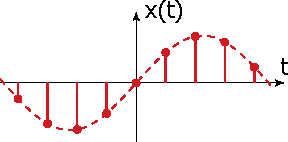
\includegraphics[width=0.65\linewidth]{chapters/03_Signale/figures/zeitdiskretessignal.pdf}
\end{minipage}
\\ \hline

\begin{minipage}[t]{\linewidth}\centering
\textbf{amplitudenkontinuierliches Signal}\\[4pt]
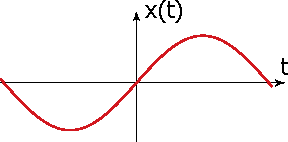
\includegraphics[width=0.65\linewidth]{chapters/03_Signale/figures/amplitudenkontinuierlichessignal.pdf}
\end{minipage}
&
\begin{minipage}[t]{\linewidth}\centering
\textbf{quantisiertes Signal}\\[4pt]
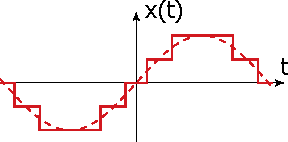
\includegraphics[width=0.65\linewidth]{chapters/03_Signale/figures/quantisiertessignal.pdf}
\end{minipage}
\\ \hline

\begin{minipage}[t]{\linewidth}\centering
\textbf{Zeit- und amplitudenkontinuierlich (Analog)}\\[4pt]
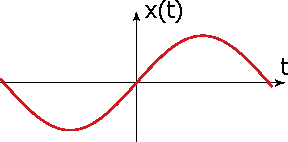
\includegraphics[width=0.65\linewidth]{chapters/03_Signale/figures/zeitamplitudenkontinuierlichessignal.pdf}
\end{minipage}
&
\begin{minipage}[t]{\linewidth}\centering
\textbf{Zeitdiskret und quantisiert (Digital)}\\[4pt]
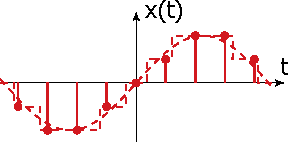
\includegraphics[width=0.65\linewidth]{chapters/03_Signale/figures/zeitdiskretquantisiert.pdf}
\end{minipage}
\\ \hline
\end{tabularx}
\end{table}
\newpage